\documentclass[8]{beamer}
\usepackage{ctex, hyperref}
\usepackage{cite}
\usepackage[T1]{fontenc}
\usepackage{hyperref}
\usefonttheme[onlymath]{serif}
\hypersetup{
    colorlinks=true,
    linkcolor=blue,
    filecolor=blue,      
    urlcolor=blue,
    citecolor=cyan,
}
% other packages
\usepackage{latexsym,amsmath,xcolor,multicol,booktabs,calligra}
\usepackage{graphicx,pstricks,listings,stackengine}

\author{Zhengyi Li}
\title{Collaborative Perception Review}
\institute[DBIV Group]{\textit{State Key Laboratory of Automotive Simulation and Control, Jilin University}}
\date{\today}
\usepackage{JilinUniv}

% defs
\def\cmd#1{\texttt{\color{red}\footnotesize $\backslash$#1}}
\def\env#1{\texttt{\color{blue}\footnotesize #1}}
\definecolor{deepblue}{rgb}{0,0,0.5}
\definecolor{deepred}{rgb}{0.6,0,0}
\definecolor{deepgreen}{rgb}{0,0.5,0}
\definecolor{halfgray}{gray}{0.55}

\lstset{
    basicstyle=\ttfamily\small,
    keywordstyle=\bfseries\color{deepblue},
    emphstyle=\ttfamily\color{deepred},    % Custom highlighting style
    stringstyle=\color{deepgreen},
    numbers=left,
    numberstyle=\small\color{halfgray},
    rulesepcolor=\color{red!20!green!20!blue!20},
    frame=shadowbox,
}
\fontsize{10}{1.5}

\begin{document}

\kaishu
\begin{frame}
    \titlepage
    \begin{figure}[htpb]
        \begin{center}
            \includegraphics[width=0.2\linewidth]{pic/Jilin_University_Logo.eps}
        \end{center}
    \end{figure}
\end{frame}

\begin{frame}
    \tableofcontents
\end{frame} 


\section{Backgroud}

\begin{frame}{Backgroud}
    \frametitle{Background}
    \begin{figure}
        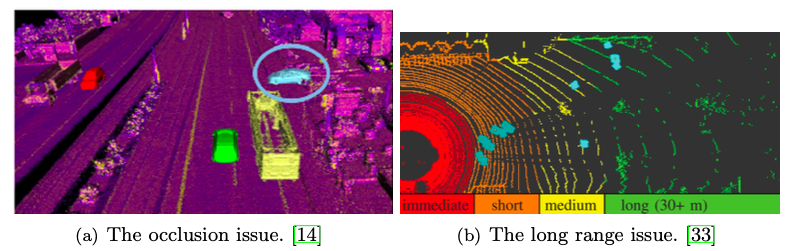
\includegraphics[width=0.7\linewidth]{pic/Intro.png}
        \caption[two_issue]{单车感知的两个局限性:a)遮挡,b)长距离衰减}
    \end{figure}
    \begin{itemize}
        \item 感知模块是自动驾驶车辆中最重要的模块之一,单车感知能力已经取得了非常大的进步,但在一定程度上已经达到了瓶颈
    \end{itemize}
\end{frame}

\begin{frame}
    \frametitle{Background}
    \begin{itemize}
        \item 为了持续提高车辆的感知能力,打破感知的局限性,在通讯技术的支持下,协同感知收到了广泛的关注\cite{ren2023collaborative}
    \end{itemize}
    

\end{frame}

\section{Related Work}
\begin{frame}
    \frametitle{Related Work}
        目前,相关工作有一定的数量和规模
        \begin{itemize}
            \footnotesize
            \item 上海交通大学\href{https://mediabrain.sjtu.edu.cn/}{MediaBrain}发表综述文章--\textit{Collaborative Perception for Autonomous Driving: Current Status and Future Trend}\cite{ren2023collaborative}
            并提出了\textit{V2VNet, DiscoNet, Who2Comm, When2Comm, Where2Comm, SyncNet}等一系列模型
            \item 法国ESIGELEC发表综述文章--\textit{Survey on Cooperative Perception in an Automotive Context}\cite{caillot2022survey}
            \item \href{https://mobility-lab.seas.ucla.edu/}{UCLA Mobility Lab}近两年在\textit{NeurIPS、ICLR、ICRA}等顶会发表并开源工作,包括数据集\textit{OPV2V}\cite{xu2022opv2v}、开源框架\textit{OpenCDA}\cite{xu2021opencda}、模型\textit{V2X-ViT}\cite{xu2022v2x}等
            \item University of North Texas的Qi Chen等先后提出了Cooper, F-Cooper模型\cite{chen2019cooper,F-Cooper}
        \end{itemize}
\end{frame}

\begin{frame}
    \frametitle{Related Work}
    \setbeamerfont{}{}
    \scriptsize
    \cite{ren2023collaborative}介绍了协同感知的基本概念,协同方式、总结了过程中的关键问题和应用,并讨论了一些行业面临的问题和挑战.\\
    协作方式和关键问题,是这篇文章写作的两条主线,也是该实验室几项工作的主线。
    \bigskip
    \begin{columns}[t]
        \begin{column}{0.5\linewidth}
            \begin{figure}
                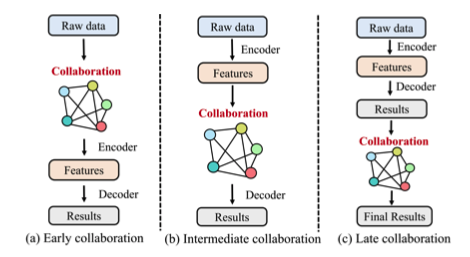
\includegraphics[width=\linewidth]{pic/Collaborative_mode.png}
                \caption[cooper_mode]{三种协同方式}
                \label{cooper_mode}
            \end{figure}
        \end{column}

        \begin{column}{0.5\linewidth}
        如图\ref{cooper_mode}所示,协作方式可以主要分为:
        \begin{itemize}
            \item \textit{Early Collaboration}--早期融合\cite{chen2019cooper, ITS_early,F-Cooper}
            \begin{itemize}
                \scriptsize
                \item 方法简单,可实施性高
                \item 占据大量的通信带宽
            \end{itemize}
            \item \textit{Late Collaboration}--后期融合
                \begin{itemize}
                    \scriptsize
                    \item 所需的通信资源较少
                    \item 容易受到丢包、延迟等噪声影响
                \end{itemize}
            \item \textit{Intermediate Collaboration}--中期融合\cite{wang2020v2vnet,liu2020who2com,liu2020when2com,li2021learning,hu_where2comm_2022}
            \begin{itemize}
                \scriptsize
                \item 在效果和通信带宽之间做了比较好的权衡
            \end{itemize}
        \end{itemize}
        \end{column}
    \end{columns}
\end{frame}

\begin{frame}[allowframebreaks]
    \frametitle{Related Work}
    \cite{ren2023collaborative}介绍了协同感知过程中的几种关键组成部分
    \begin{itemize}
        \item 协作图:
        \begin{itemize}
            \item 协作图是构建整个过程的重要工具,在一些工作中,将车辆或路侧设备作为图的节点,通信关系作为图的边,对过程进行建模。
            \item 针对于协作图的研究,是MediaBrain几篇工作的主要研究内容,例如\cite{wang2020v2vnet,li2021learning,liu2020who2com, liu2020when2com, hu_where2comm_2022}
            都是针对协作图进行研究,优化目标为:\textbf{使用更少的通信带宽来达到更强的感知能力。}
        \end{itemize}
        \item 信息对齐:
        \begin{itemize}
            \item 由于多个智能体信息的时空不对称性,信息对齐是协同感知重要的组成部分之一
            \item MediaBrain提出了\textit{SyncNet}\cite{lei2022latency},补偿了通信延时对整个模型造成的影响
            \item UCLA-Mobility Lab提出的\textit{V2X-ViT}\cite{xu2022v2x}将通信延迟作为Transformer\cite{transformer}结构中的
            \textit{Position Embedding}输入,对通信延时进行补偿
        \end{itemize}
        \item 信息融合:
        \begin{itemize}
            \item 收到多个智能体信息后,单车的信息融合是整个过程中最重要的环节。
            \item \textit{CommNet}\cite{CommNet}将收到的信息通过均值操作合并到一起,以\textit{VAIN}\cite{VAIN}为代表的注意力机制在得到的广泛的应用
        \end{itemize}
    \end{itemize}
\end{frame}

\begin{frame}
    \frametitle{Related Work}
    Related Work Summary:
    \begin{itemize}
        \item \cite{ren2023collaborative,caillot2022survey}两篇综述中,相关工作大多均为2020年后发表
        \item \textit{Intermediate Collaboration}是学术研究中使用最广泛的一种方式
        \item MediaBrain与UCLA Mobility Lab的工作最为先进和成体系,但两者侧重点不同
        \item MediaBrain与UCLA-Mobility Lab工作均开源数据集和开放源码
    \end{itemize}
\end{frame}

\section{Baseline}
\subsection{MediaBrain Lab}
\begin{frame}
    \frametitle{MediaBrain -- V2X-Sim\cite{Li_2021_RAL}}
    \begin{columns}
        \begin{column}{ 0.5\linewidth}
            \begin{figure}
                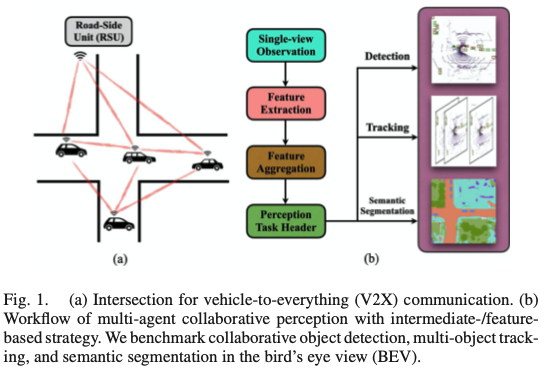
\includegraphics[width=\linewidth]{pic/V2XSim.png}
            \end{figure}
        \end{column}

        \begin{column}{0.5\linewidth}
            V2X-Sim是基于仿真场景的,协同感知数据集,包括:
            \begin{itemize}
                \item 路侧传感器和车辆传感器数据
                \item 多类型传感器数据
                \item 多种感知任务的Ground Truth标签
            \end{itemize}
        \end{column}
    \end{columns}
\bigskip
Basebone:
\begin{columns}
    \begin{column}{0.5\linewidth}
        \begin{itemize}
            \item Encoder
            \item Collaboration Graph
        \end{itemize}
    \end{column}

    \begin{column}{0.5\linewidth}
        \begin{itemize}
            \item Decoder
            \item Output Header
        \end{itemize}
    \end{column}
\end{columns}
\end{frame}

\begin{frame}
    \begin{figure}
        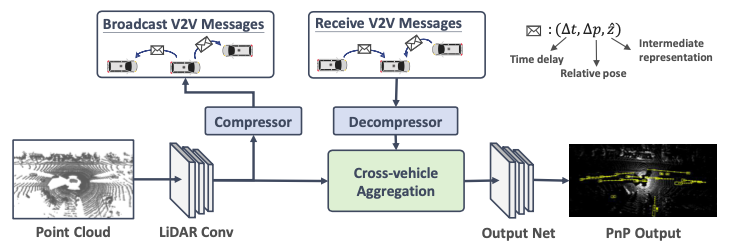
\includegraphics[width=0.7\linewidth]{pic/V2Vnet.png}
    \end{figure}
    \frametitle{MediaBrain -- V2VNet\cite{wang2020v2vnet}}
        \textit{V2VNet}是一种利用\textit{GNN}聚合信息的感知预测(\textit{P\&P})模型 
        \bigskip
        \textbf{Key Words}: \textit{GNN}, \textit{ConvRNN}
    \textit{V2VNet}主要分为三个阶段:
    \begin{itemize}
        \footnotesize
        \item 数据预处理(\textit{CNNs})与压缩(\textit{SOTA算法})
        \item 信息融合:
            \begin{itemize}
                \item 信息解压缩
                \item 使用\textit{GNN}进行信息融合,以满足不同车辆的空间位置与时间的变化
            \end{itemize}
        \item 结果输出:\textit{End-to-End}输出感知与预测结果
    \end{itemize}
\end{frame}

\begin{frame}
    \frametitle{MediaBrain -- DiscoNet\cite{li2021learning}}
        \cite{li2021learning}提出了一种基于知识蒸馏\cite{hinton2015distilling}的可训练的协作图,使用矩阵表示,
        矩阵上的值表示节点之间传递消息的权重
        \bigskip
        \begin{itemize}
            \item 教师模型使用\textit{Early Collaboration},使用全局信息进行感知
            \item 学生模型分为四个部分:
            \begin{itemize}
                \item 特征编码:将\textit{BEV}经过\textit{CNNs}得到\textit{Feature Map}
                \item 特征压缩:使用$1\times 1 conv$进行特征压缩
                \item 协作图构建:
                \begin{itemize}
                    \item 信息传递
                    \item 得到图注意力
                    \item 信息合并
                \end{itemize}
                \item 解码并输出结果:使用$CNNs$解码并输出结果
            \end{itemize}
        \end{itemize}
\end{frame}

\begin{frame}
    \frametitle{MediaBrain -- DiscoNet\cite{li2021learning}}
    \begin{figure}
        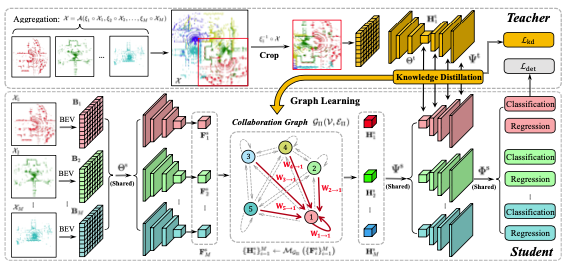
\includegraphics[width=0.6\linewidth]{pic/DiscoNet.png}
    \end{figure}
        \begin{itemize}
        \footnotesize
        \item Message Transmission:每个智能体将压缩后的$Feature Map$传输给其他智能体
        \item Message Attention:
        \begin{itemize}
            \footnotesize
            \item 智能体$i$接收智能体$j$的信息$F_j$,并基于位置,将信息$F_j$变换到$agent_i$的坐标系下$F_{j\rightarrow i}=\Gamma_{j\rightarrow i}(F_i) $
            \item 使用边编码器将边编码$W_{j\rightarrow i} = \Pi (F_{j \rightarrow i}, F_i)$
            \item 使用$1\times 1 convs$降维得到$Attention$数值
        \end{itemize}
        \item Message Aggregation:每个智能体根据$Attention$权重得到合并后的$Feature Map$  
     \end{itemize}
\end{frame}

\begin{frame}
    \frametitle{MediaBrain -- Who2com\cite{liu2020who2com}}
    \cite{liu2020who2com}提出了一种多阶段、握手机制(Multi-stage Handshake Communication)的通信方式,当智能体发送
    请求,其他智能体接收信息并计算匹配程度,自动选择一个或多个智能体进行协同,大大减少了带宽的消耗,包含三个部分:
    \begin{columns}
        \begin{column}{0.3\linewidth}
            \begin{itemize}
                \item $Request$
            \end{itemize}
        \end{column}

        \begin{column}{0.3\linewidth}
            \begin{itemize}
                \item $Match$
            \end{itemize}
        \end{column}

        \begin{column}{0.3\linewidth}
            \begin{itemize}
                \item $Connect$
            \end{itemize}
        \end{column}
    \end{columns}
    \begin{figure}
        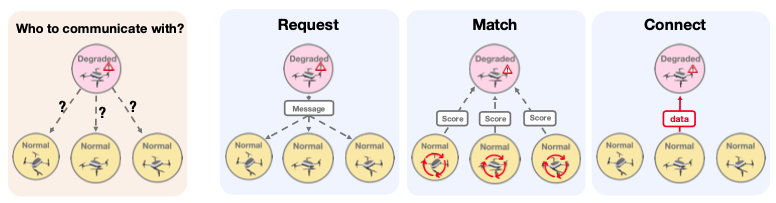
\includegraphics[width=\linewidth]{pic/Who2com.png}
    \end{figure}

\end{frame}

\begin{frame}
    \frametitle{MediaBrain -- Who2com\cite{liu2020who2com}}
    \begin{itemize}
        \item Request: $Agent_i$发送压缩后的$Request: \nu_i = G^j_m(\widetilde{x} _i;\theta_m)$
        \item Match: 匹配分数$s_{ij}=\Phi(\mu_i,\kappa_j), \kappa_j = G_k^j (x_j;\theta_k)$
        \begin{itemize}
            \item 其中,$\Phi = \nu_j^T W_a \kappa_i$,应是根据\cite{transformer}中$Self-Attention$计算相关度的方法
        \end{itemize}
        \item Connect: 连接并传送信息
    \end{itemize}
    \bigskip
    \bigskip
    训练过程中不以最优匹配为目标,以最大化感知能力为目标,克服了该问题数据集缺少的问题
\end{frame}

\begin{frame}
    \frametitle{MediaBrain -- When2comm\cite{liu2020when2com}}
        $When2com$在$Who2com$的基础上,增加了对通信触发的判断(类似于事件触发),进一步减少了通信带宽的消耗。\\
    
    \begin{figure}
        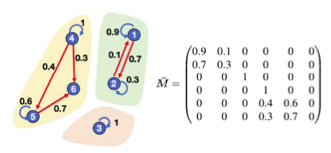
\includegraphics[width=0.5\linewidth]{pic/When2com.png}
    \end{figure}

    在$Who2com$的三段上,$When2com$基于$Self-Attention$和$Cross-Attention$生成一个矩阵,表示每个智能体
    接收不同其他智能体的权重,当
    $$ m_{i, i} = 1 $$
    时,$Agent_i$不需要接收其他智能体的信息

\end{frame}

\begin{frame}
    \frametitle{MediaBrain -- SyncNet}

    

\end{frame}

\subsection{UCLA-Mobility Lab}
\begin{frame}
    \frametitle{UCLA-Mobility Lab -- OPV2V}

    

\end{frame}

\begin{frame}
    \frametitle{UCLA-Mobility Lab -- OpenCDA}

    

\end{frame}

\begin{frame}
    \frametitle{UCLA-Mobility Lab -- V2X-ViT}

    

\end{frame}

\begin{frame}
    \frametitle{UCLA-Mobility Lab -- Bridging---}

    

\end{frame}
% \section{研究内容}

% \subsection{美化主题}

% \begin{frame}{这一份主题与原始的THU Beamer Theme区别在于}
%     \begin{itemize}
%         \item 顶栏的小点变成一行而不是多行
%         \item 中文采用楷书
%         \item 由于吉大校徽的配色有点艳丽,本文主题色采用了RGB\#336699,主题色可在JilinUniv.sty文件中修改
%         \item 更多该模板的功能可以参考 \url{https://www.latexstudio.net/archives/4051.html}
%     \end{itemize}
% \end{frame}

% \subsection{如何更好地做Beamer}

% \begin{frame}{Why Beamer}
%     \begin{itemize}
%         \item \LaTeX 广泛用于学术界,期刊会议论文模板
%     \end{itemize}
%     \begin{table}[h]
%         \centering
%         \begin{tabular}{c|c}
%             Microsoft\textsuperscript{\textregistered}  Word & \LaTeX \\
%             \hline
%             文字处理工具 & 专业排版软件 \\
%             容易上手,简单直观 & 容易上手 \\
%             所见即所得 & 所见即所想,所想即所得 \\
%             高级功能不易掌握 & 进阶难,但一般用不到 \\
%             处理长文档需要丰富经验 & 和短文档处理基本无异 \\
%             花费大量时间调格式 & 无需担心格式,专心作者内容 \\
%             公式排版差强人意 & 尤其擅长公式排版 \\
%             二进制格式,兼容性差 & 文本文件,易读、稳定 \\
%             付费商业许可 & 自由免费使用 \\
%         \end{tabular}
%     \end{table}
% \end{frame}

% \begin{frame}{排版举例}
%     \begin{exampleblock}{无编号公式} % 加 * 
%         \begin{equation*}
%             J(\theta) = \mathbb{E}_{\pi_\theta}[G_t] = \sum_{s\in\mathcal{S}} d^\pi (s)V^\pi(s)=\sum_{s\in\mathcal{S}} d^\pi(s)\sum_{a\in\mathcal{A}}\pi_\theta(a|s)Q^\pi(s,a)
%         \end{equation*}
%     \end{exampleblock}
%     \begin{exampleblock}{多行多列公式\footnote{如果公式中有文字出现,请用 $\backslash$mathrm\{\} 或者 $\backslash$text\{\} 包含,不然就会变成 $clip$,在公式里看起来比 $\mathrm{clip}$ 丑非常多。}}
%         % 使用 & 分隔
%         \begin{align}
%             Q_\mathrm{target}&=r+\gamma Q^\pi(s^\prime, \pi_\theta(s^\prime)+\epsilon)\\
%             \epsilon&\sim\mathrm{clip}(\mathcal{N}(0, \sigma), -c, c)\nonumber
%         \end{align}
%     \end{exampleblock}
% \end{frame}

% \begin{frame}
%     \begin{exampleblock}{编号多行公式}
%         % Taken from Mathmode.tex
%         \begin{multline}
%             A=\lim_{n\rightarrow\infty}\Delta x\left(a^{2}+\left(a^{2}+2a\Delta x+\left(\Delta x\right)^{2}\right)\right.\label{eq:reset}\\
%             +\left(a^{2}+2\cdot2a\Delta x+2^{2}\left(\Delta x\right)^{2}\right)\\
%             +\left(a^{2}+2\cdot3a\Delta x+3^{2}\left(\Delta x\right)^{2}\right)\\
%             +\ldots\\
%             \left.+\left(a^{2}+2\cdot(n-1)a\Delta x+(n-1)^{2}\left(\Delta x\right)^{2}\right)\right)\\
%             =\frac{1}{3}\left(b^{3}-a^{3}\right)
%         \end{multline}
%     \end{exampleblock}
% \end{frame}

% \begin{frame}{图形与分栏}
%     % From thuthesis user guide.
%     \begin{minipage}[c]{0.3\linewidth}
%         \psset{unit=0.8cm}
%         \begin{pspicture}(-1.75,-3)(3.25,4)
%             \psline[linewidth=0.25pt](0,0)(0,4)
%             \rput[tl]{0}(0.2,2){$\vec e_z$}
%             \rput[tr]{0}(-0.9,1.4){$\vec e$}
%             \rput[tl]{0}(2.8,-1.1){$\vec C_{ptm{ext}}$}
%             \rput[br]{0}(-0.3,2.1){$\theta$}
%             \rput{25}(0,0){%
%             \psframe[fillstyle=solid,fillcolor=lightgray,linewidth=.8pt](-0.1,-3.2)(0.1,0)}
%             \rput{25}(0,0){%
%             \psellipse[fillstyle=solid,fillcolor=yellow,linewidth=3pt](0,0)(1.5,0.5)}
%             \rput{25}(0,0){%
%             \psframe[fillstyle=solid,fillcolor=lightgray,linewidth=.8pt](-0.1,0)(0.1,3.2)}
%             \rput{25}(0,0){\psline[linecolor=red,linewidth=1.5pt]{->}(0,0)(0.,2)}
% %           \psRotation{0}(0,3.5){$\dot\phi$}
% %           \psRotation{25}(-1.2,2.6){$\dot\psi$}
%             \psline[linecolor=red,linewidth=1.25pt]{->}(0,0)(0,2)
%             \psline[linecolor=red,linewidth=1.25pt]{->}(0,0)(3,-1)
%             \psline[linecolor=red,linewidth=1.25pt]{->}(0,0)(2.85,-0.95)
%             \psarc{->}{2.1}{90}{112.5}
%             \rput[bl](.1,.01){C}
%         \end{pspicture}
%     \end{minipage}\hspace{1cm}
%     \begin{minipage}{0.5\linewidth}
%         \medskip
%         %\hspace{2cm}
%         \begin{figure}[h]
%             \centering
%             \includegraphics[height=.4\textheight]{pic/dtmf.pdf}
%         \end{figure}
%     \end{minipage}
% \end{frame}

% \begin{frame}[fragile]{\LaTeX{} 常用命令}
%     \begin{exampleblock}{命令}
%         \centering
%         \footnotesize
%         \begin{tabular}{llll}
%             \cmd{chapter} & \cmd{section} & \cmd{subsection} & \cmd{paragraph} \\
%             章 & 节 & 小节 & 带题头段落 \\\hline
%             \cmd{centering} & \cmd{emph} & \cmd{verb} & \cmd{url} \\
%             居中对齐 & 强调 & 原样输出 & 超链接 \\\hline
%             \cmd{footnote} & \cmd{item} & \cmd{caption} & \cmd{includegraphics} \\
%             脚注 & 列表条目 & 标题 & 插入图片 \\\hline
%             \cmd{label} & \cmd{cite} & \cmd{ref} \\
%             标号 & 引用参考文献 & 引用图表公式等\\\hline
%         \end{tabular}
%     \end{exampleblock}
%     \begin{exampleblock}{环境}
%         \centering
%         \footnotesize
%         \begin{tabular}{lll}
%             \env{table} & \env{figure} & \env{equation}\\
%             表格 & 图片 & 公式 \\\hline
%             \env{itemize} & \env{enumerate} & \env{description}\\
%             无编号列表 & 编号列表 & 描述 \\\hline
%         \end{tabular}
%     \end{exampleblock}
% \end{frame}

% \begin{frame}[fragile]{\LaTeX{} 环境命令举例}
%     \begin{minipage}{0.5\linewidth}
% \begin{lstlisting}[language=TeX]
% \begin{itemize}
%   \item A \item B
%   \item C
%   \begin{itemize}
%     \item C-1
%   \end{itemize}
% \end{itemize}
% \end{lstlisting}
%     \end{minipage}\hspace{1cm}
%     \begin{minipage}{0.3\linewidth}
%         \begin{itemize}
%             \item A
%             \item B
%             \item C
%             \begin{itemize}
%                 \item C-1
%             \end{itemize}
%         \end{itemize}
%     \end{minipage}
%     \medskip
%     \pause
%     \begin{minipage}{0.5\linewidth}
% \begin{lstlisting}[language=TeX]
% \begin{enumerate}
%   \item 白山 \item 旭日
%   \item 黑水
%   \begin{itemize}
%     \item[n+e] 红太阳
%   \end{itemize}
% \end{enumerate}
% \end{lstlisting}
%     \end{minipage}\hspace{1cm}
%     \begin{minipage}{0.3\linewidth}
%         \begin{enumerate}
%             \item 白山
%             \item 旭日
%             \item 黑水
%             \begin{itemize}
%                 \item[n+e] 红太阳
%             \end{itemize}
%         \end{enumerate}
%     \end{minipage}
% \end{frame}

% \begin{frame}[fragile]{\LaTeX{} 数学公式}
%     \begin{columns}
%         \begin{column}{.55\textwidth}
% \begin{lstlisting}[language=TeX]
% $V = \frac{4}{3}\pi r^3$

% \[
%   V = \frac{4}{3}\pi r^3
% \]

% \begin{equation}
%   \label{eq:vsphere}
%   V = \frac{4}{3}\pi r^3
% \end{equation}
% \end{lstlisting}
%         \end{column}
%         \begin{column}{.4\textwidth}
%             $V = \frac{4}{3}\pi r^3$
%             \[
%                 V = \frac{4}{3}\pi r^3
%             \]
%             \begin{equation}
%                 \label{eq:vsphere}
%                 V = \frac{4}{3}\pi r^3
%             \end{equation}
%         \end{column}
%     \end{columns}
%     \begin{itemize}
%         \item 更多内容请看 \href{https://zh.wikipedia.org/wiki/Help:数学公式}{\color{purple}{这里}}
%     \end{itemize}
% \end{frame}

% \begin{frame}[fragile]
%     \begin{columns}
%         \column{.6\textwidth}
% \begin{lstlisting}[language=TeX]
%     \begin{table}[htbp]
%       \caption{编号与含义}
%       \label{tab:number}
%       \centering
%       \begin{tabular}{cl}
%         \toprule
%         编号 & 含义 \\
%         \midrule
%         1 & 4.0 \\
%         2 & 3.7 \\
%         \bottomrule
%       \end{tabular}
%     \end{table}
%     公式~(\ref{eq:vsphere}) 的
%     编号与含义请参见
%     表~\ref{tab:number}。
% \end{lstlisting}
%         \column{.4\textwidth}
%         \begin{table}[htpb]
%             \centering
%             \caption{编号与含义}
%             \label{tab:number}
%             \begin{tabular}{cl}\toprule
%                 编号 & 含义 \\\midrule
%                 1 & 4.0\\
%                 2 & 3.7\\\bottomrule
%             \end{tabular}
%         \end{table}
%         \normalsize 公式~(\ref{eq:vsphere})的编号与含义请参见表~\ref{tab:number}。
%     \end{columns}
% \end{frame}

% \begin{frame}{作图}
%     \begin{itemize}
%         \item 矢量图 eps, ps, pdf
%         \begin{itemize}
%             \item METAPOST, pstricks, pgf $\ldots$
%             \item Xfig, Dia, Visio, Inkscape $\ldots$
%             \item Matlab / Excel 等保存为 pdf
%         \end{itemize}
%         \item 标量图 png, jpg, tiff $\ldots$
%         \begin{itemize}
%             \item 提高清晰度,避免发虚
%             \item 应尽量避免使用
%         \end{itemize}
%     \end{itemize}
%     \begin{figure}[htpb]
%         \centering
%         \includegraphics[width=0.2\linewidth]{pic/Jilin_University_Logo.eps}
%         \caption{这个校徽就是矢量图}
%     \end{figure}
% \end{frame}

% \section{计划进度}
% \begin{frame}
%     \begin{itemize}
%         \item 我是一只酸菜鱼
%         \item 又酸又菜又多余
%         \item 我是一只黄焖鸡
%         \item 又黄又焖又辣鸡
%     \end{itemize}
% \end{frame}

\section{Reference}

\begin{frame}[allowframebreaks]
    \frametitle{Reference}
    \tiny
    \bibliography{ref}
    \bibliographystyle{unsrt}
    % 如果参考文献太多的话,可以像下面这样调整字体:
    % \tiny\bibliographystyle{alpha}
\end{frame}

\begin{frame}
    \begin{center}
        {\Huge\calligra Thanks!}
    \end{center}
\end{frame}

\end{document}